% +++
% latex="texfot lualatex-dev"
% +++
\documentclass[body]{subfiles}
\begin{document}
\chapter{実験結果}

実験結果(図を貼る)。

\section{\(S=1366\hmu{W/m^2}\)の結果}
地表面温度、子午面温度分布、東西風、時系列

\section{??? の太陽定数依存性}

\section{南北熱輸送の太陽定数依存性}

\begin{figure}[t]
	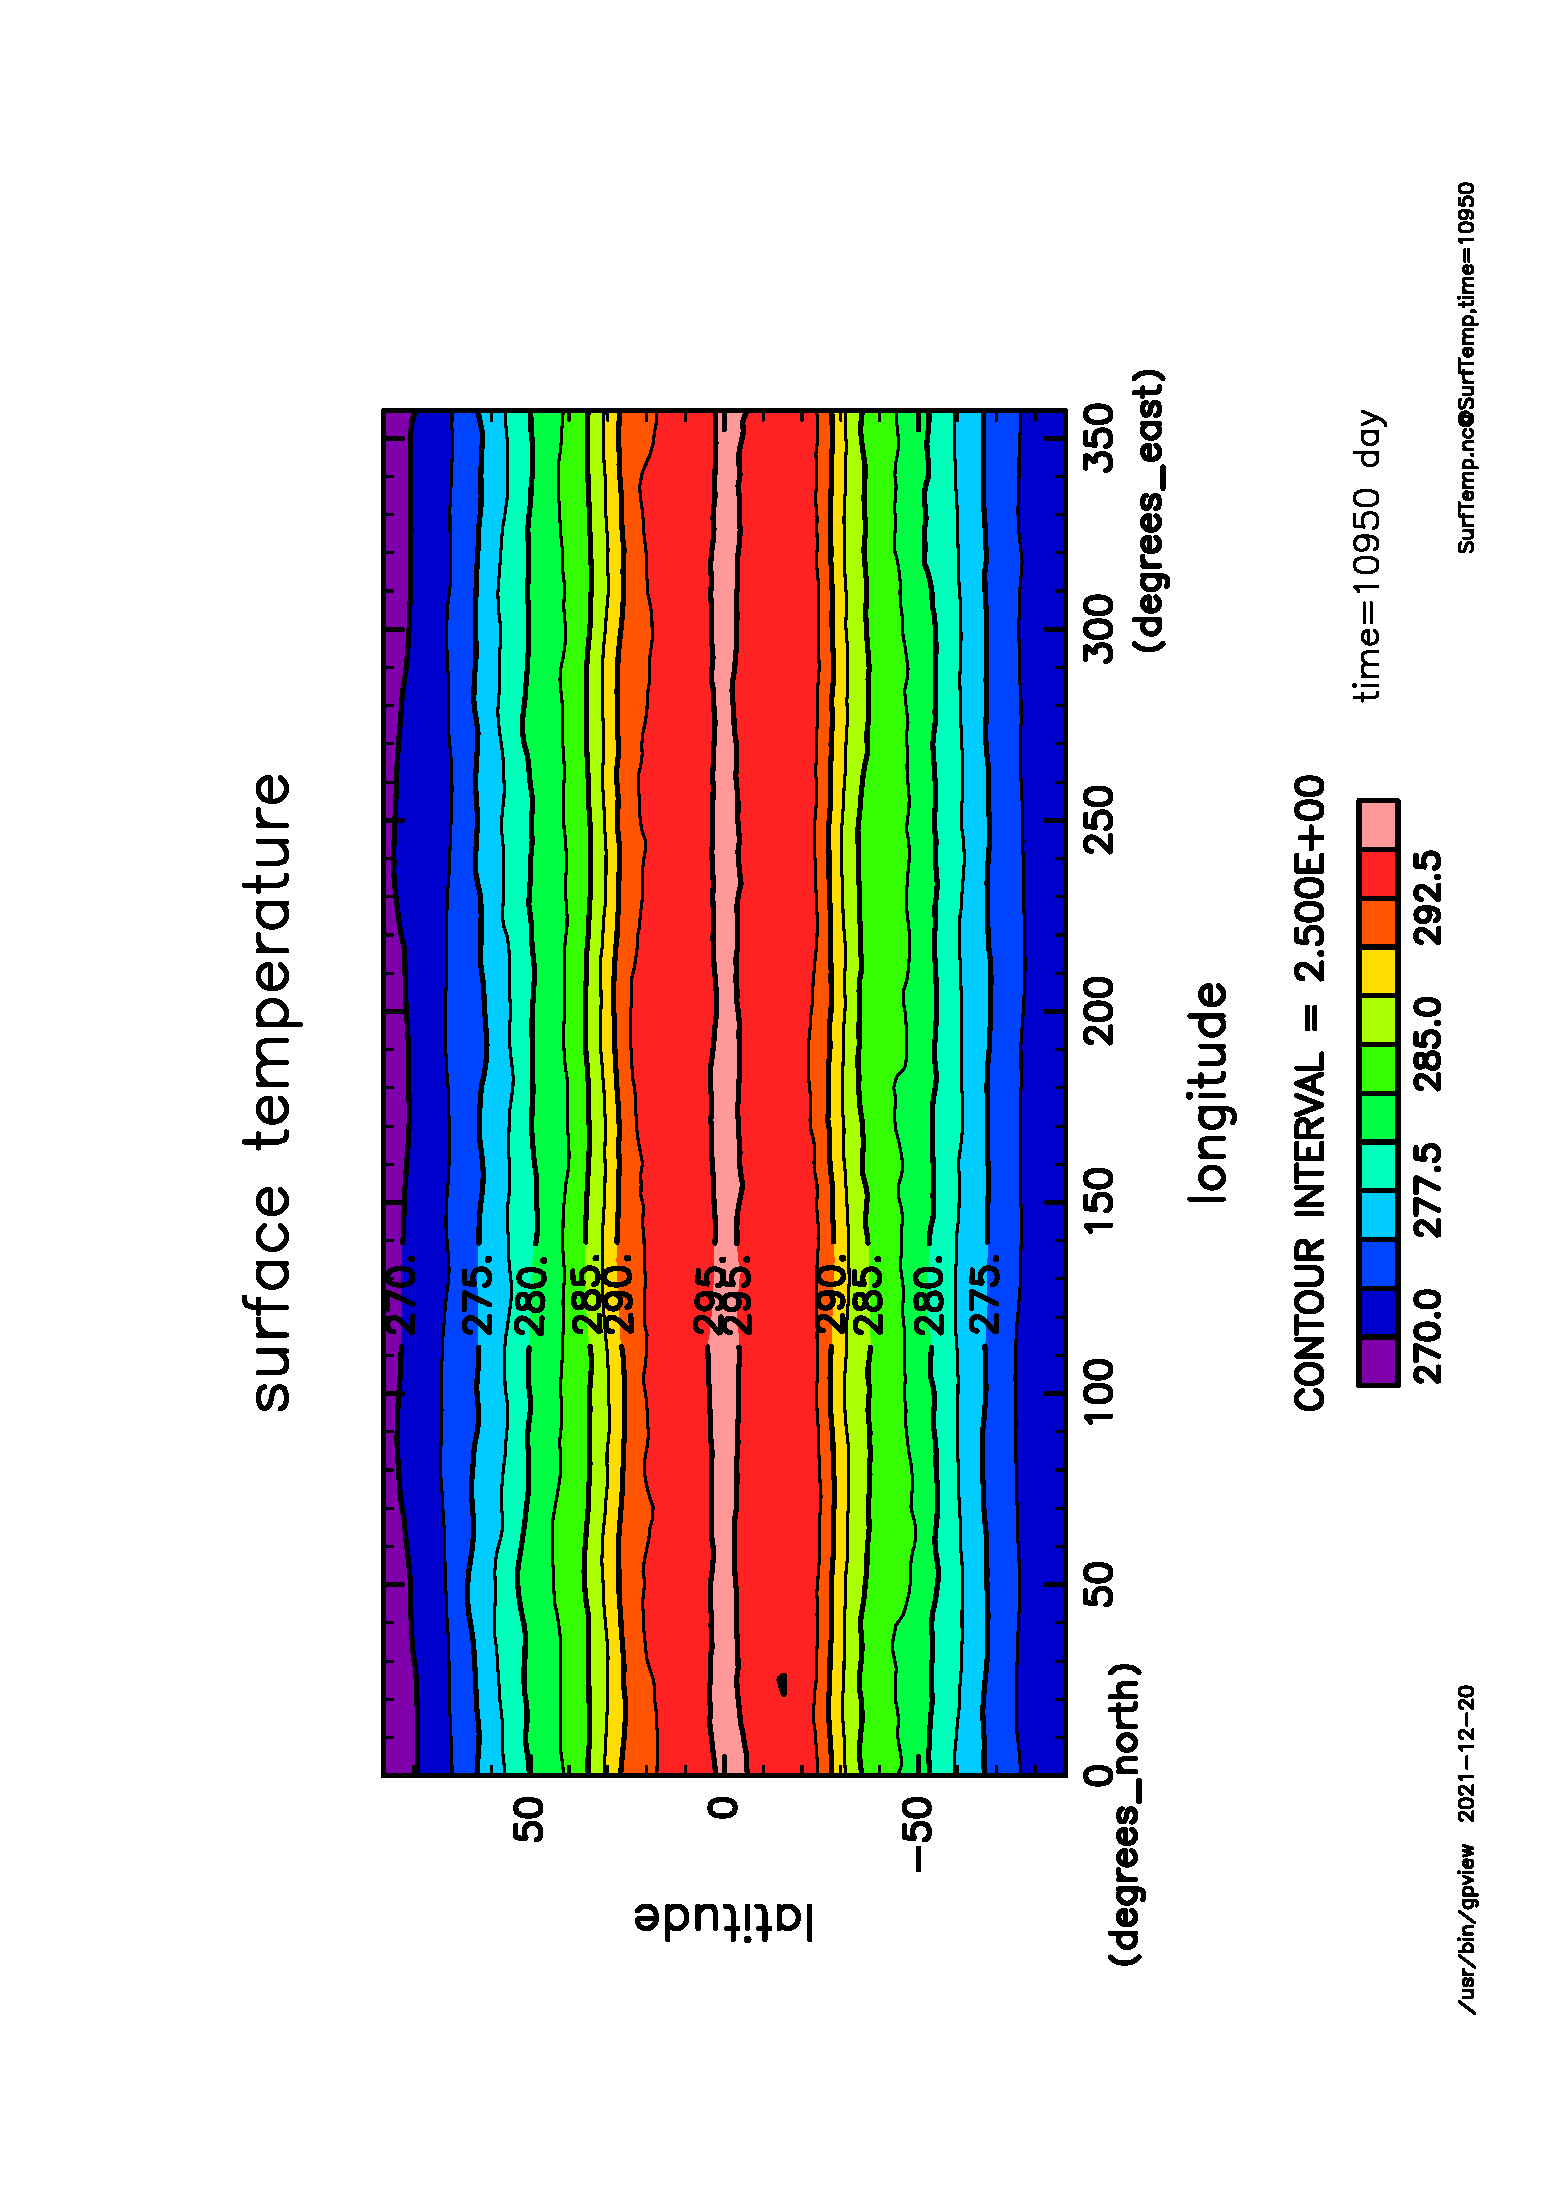
\includegraphics[height=\textwidth,angle=-90]{S1366SurfTemp,time=10950.pdf}
	\caption{\(S=1366\hmu{W/m^2}\) 30 年目の地表面温度}
\end{figure}
\begin{figure}[t]
	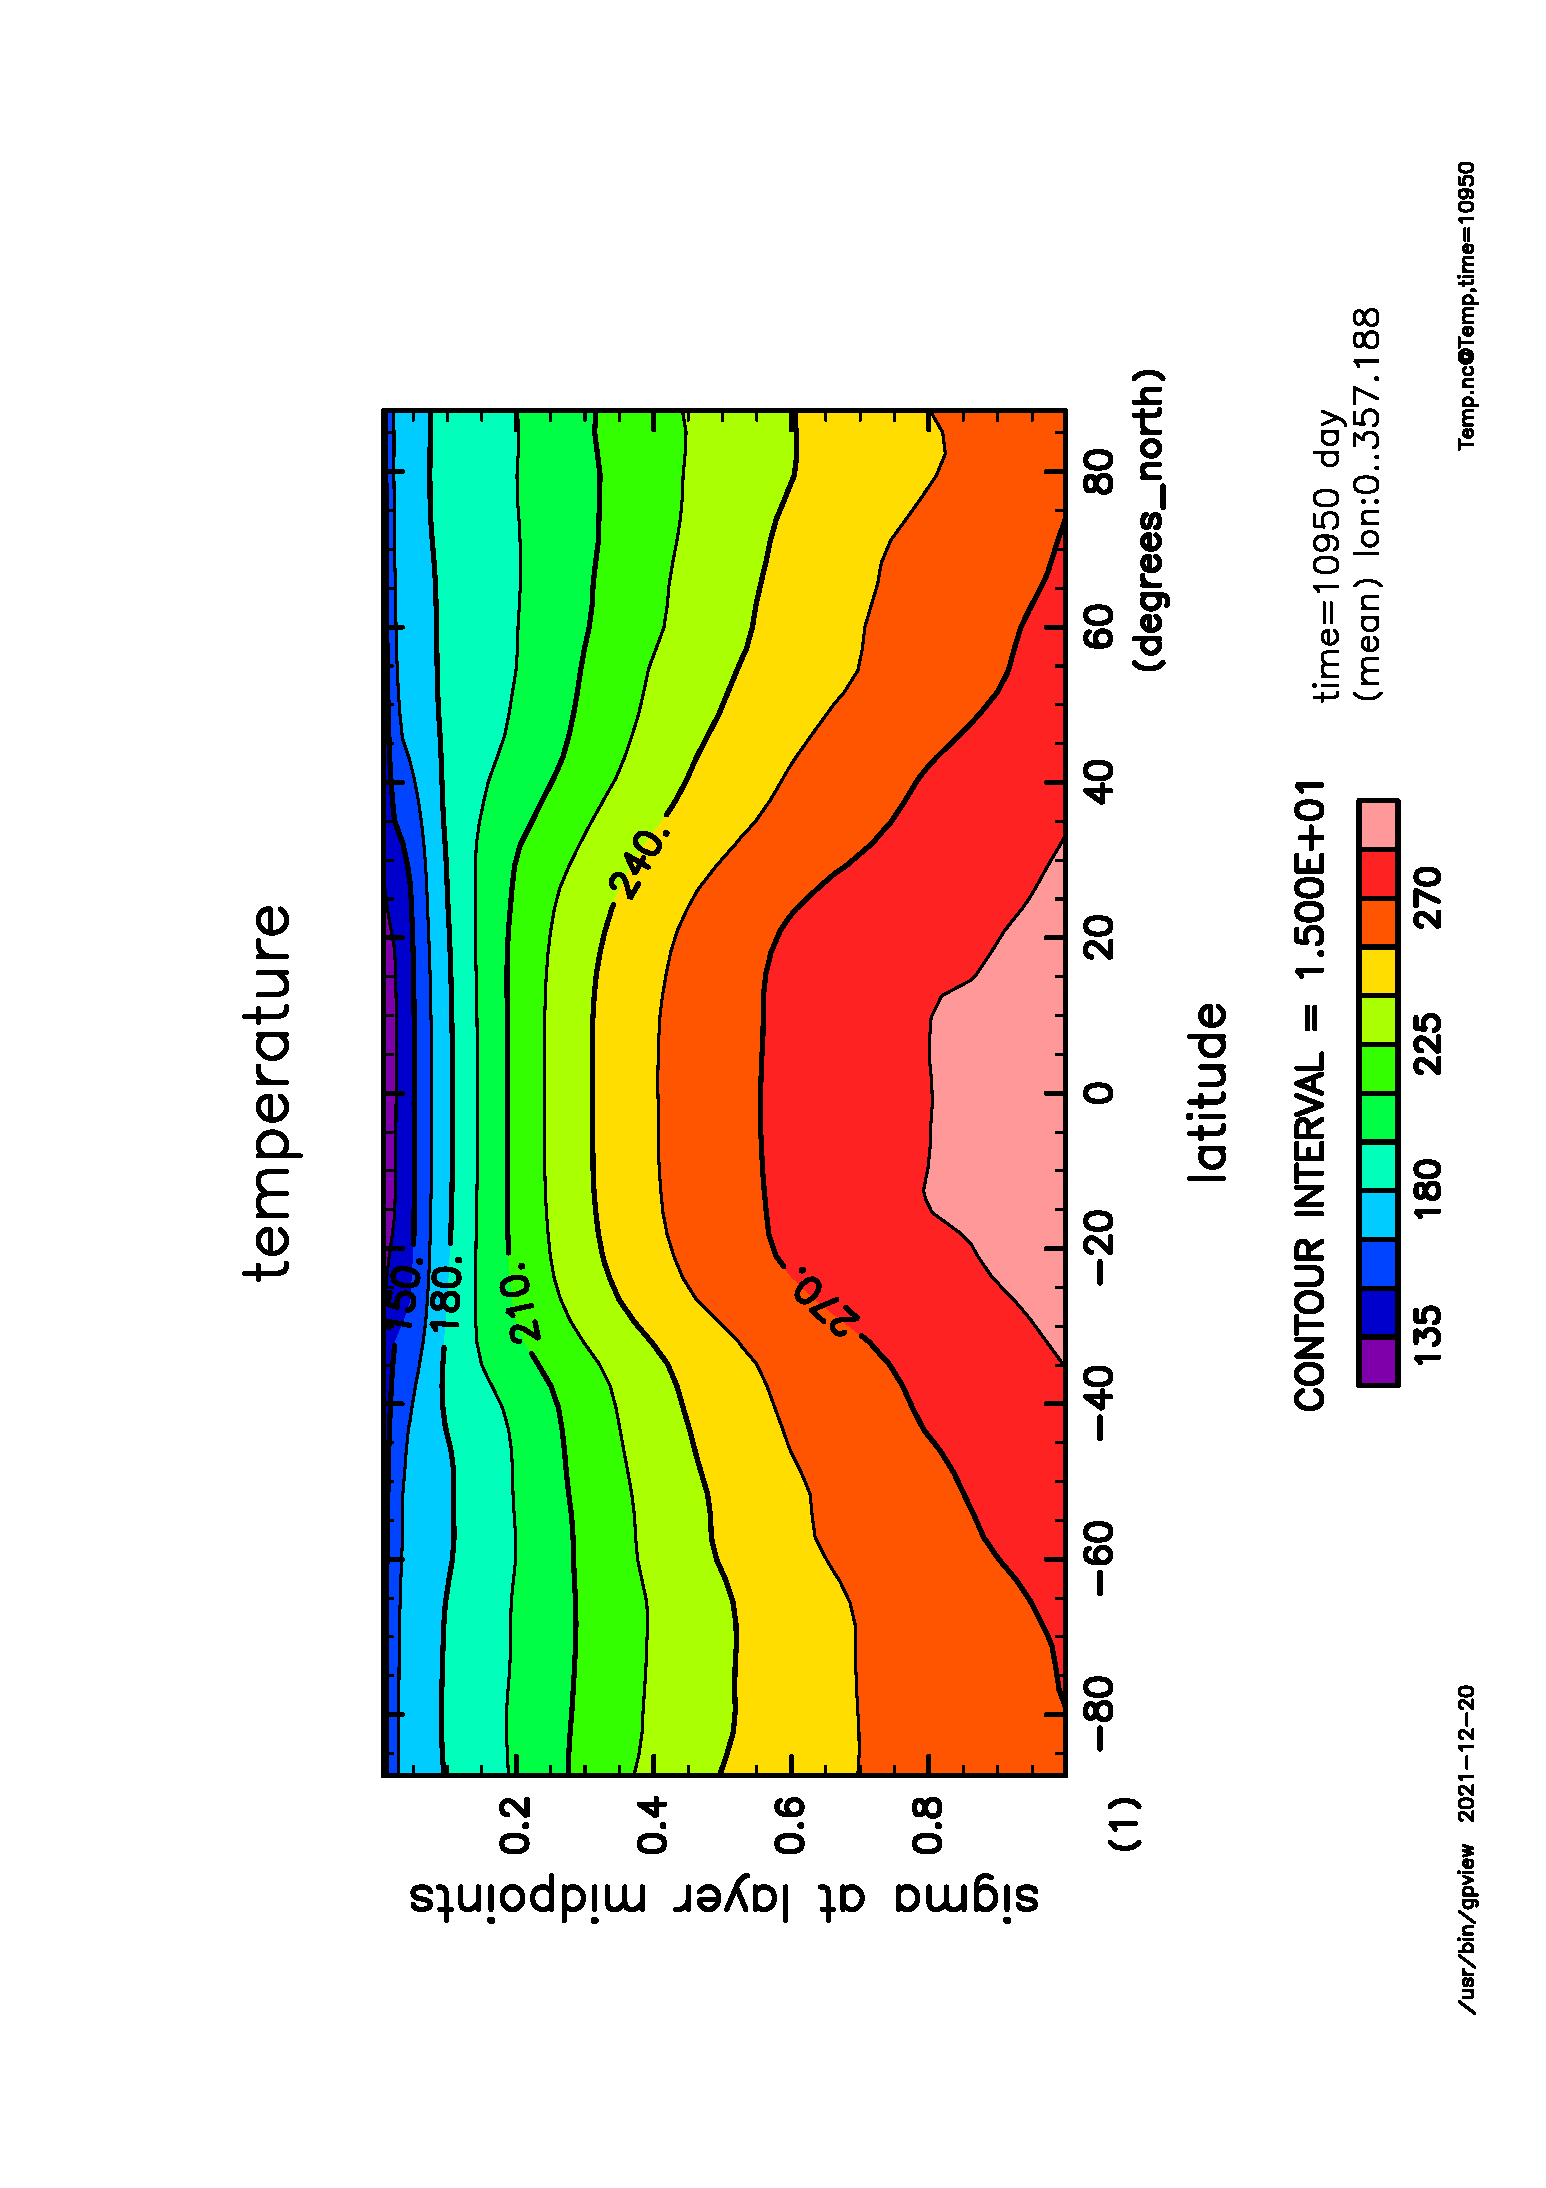
\includegraphics[height=\textwidth,angle=-90]{S1366Temp,time=10950.pdf}
	\caption{\(S=1366\hmu{W/m^2}\) 30 年目の子午面温度分布}
\end{figure}
\begin{figure}[t]
	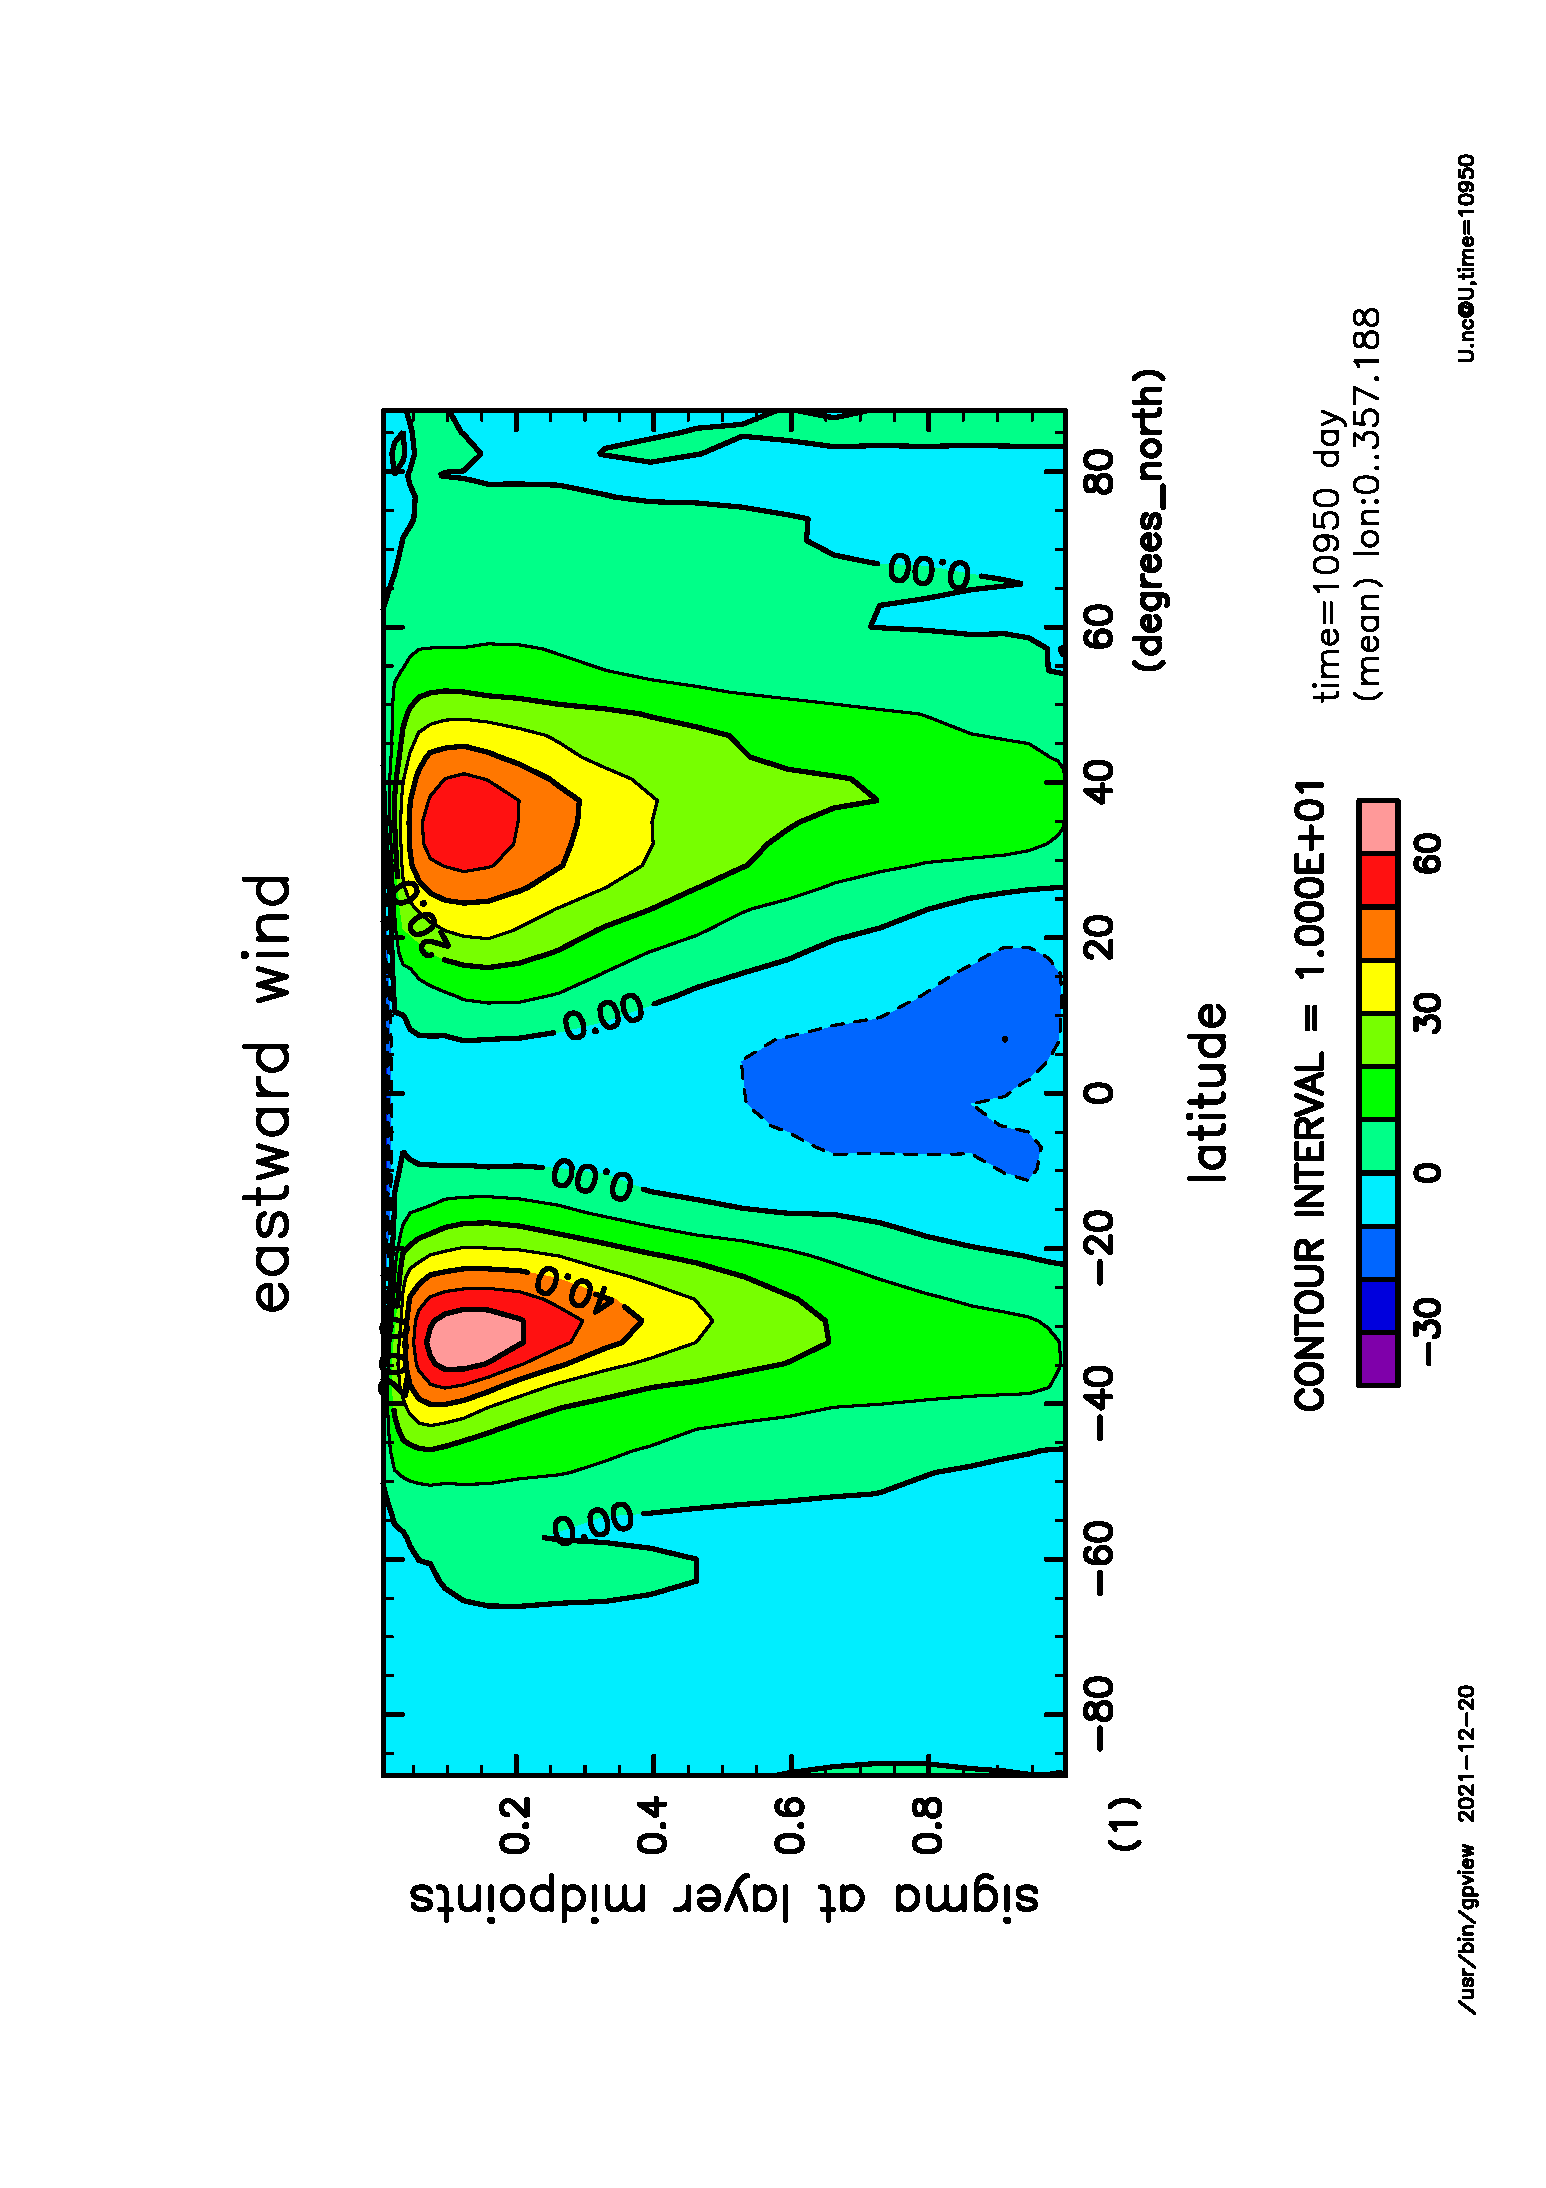
\includegraphics[height=\textwidth,angle=-90]{S1366U,time=10950.pdf}
	\caption{\(S=1366\hmu{W/m^2}\) 30 年目の東西風}
\end{figure}
\begin{figure}[t]
	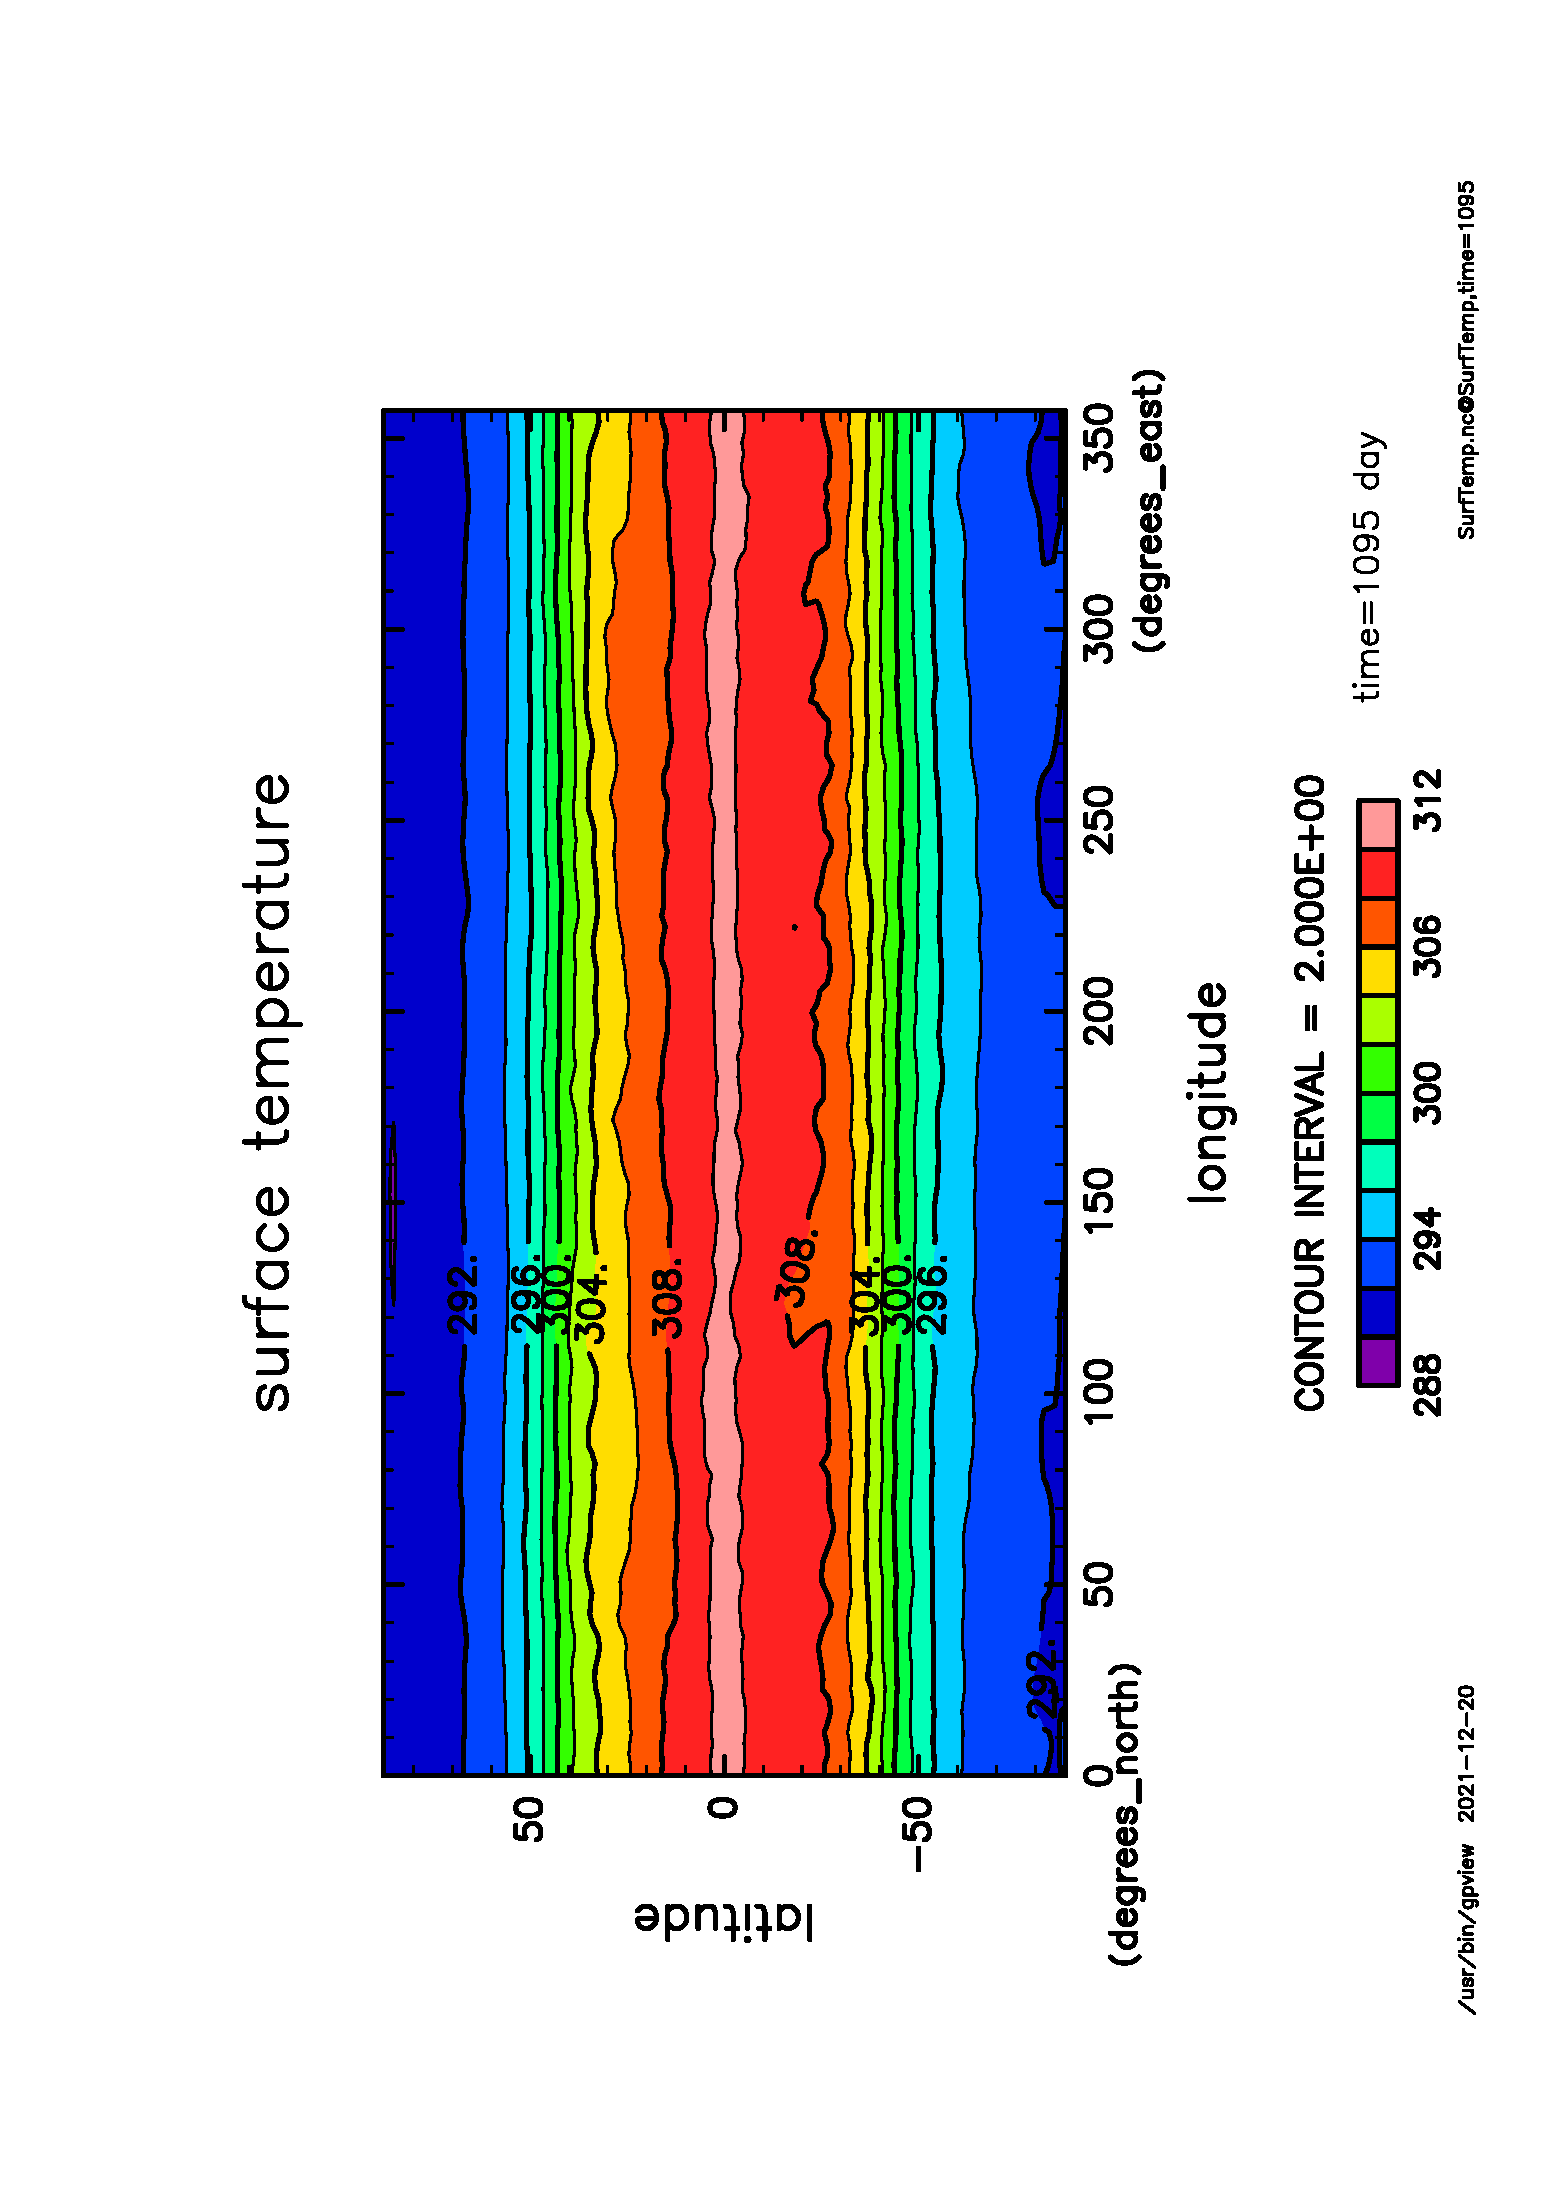
\includegraphics[height=\textwidth,angle=-90]{S2000SurfTemp,time=1095.pdf}
	\caption{\(S=2000\hmu{W/m^2}\) 3 年目の地表面温度}
\end{figure}
\begin{figure}[t]
	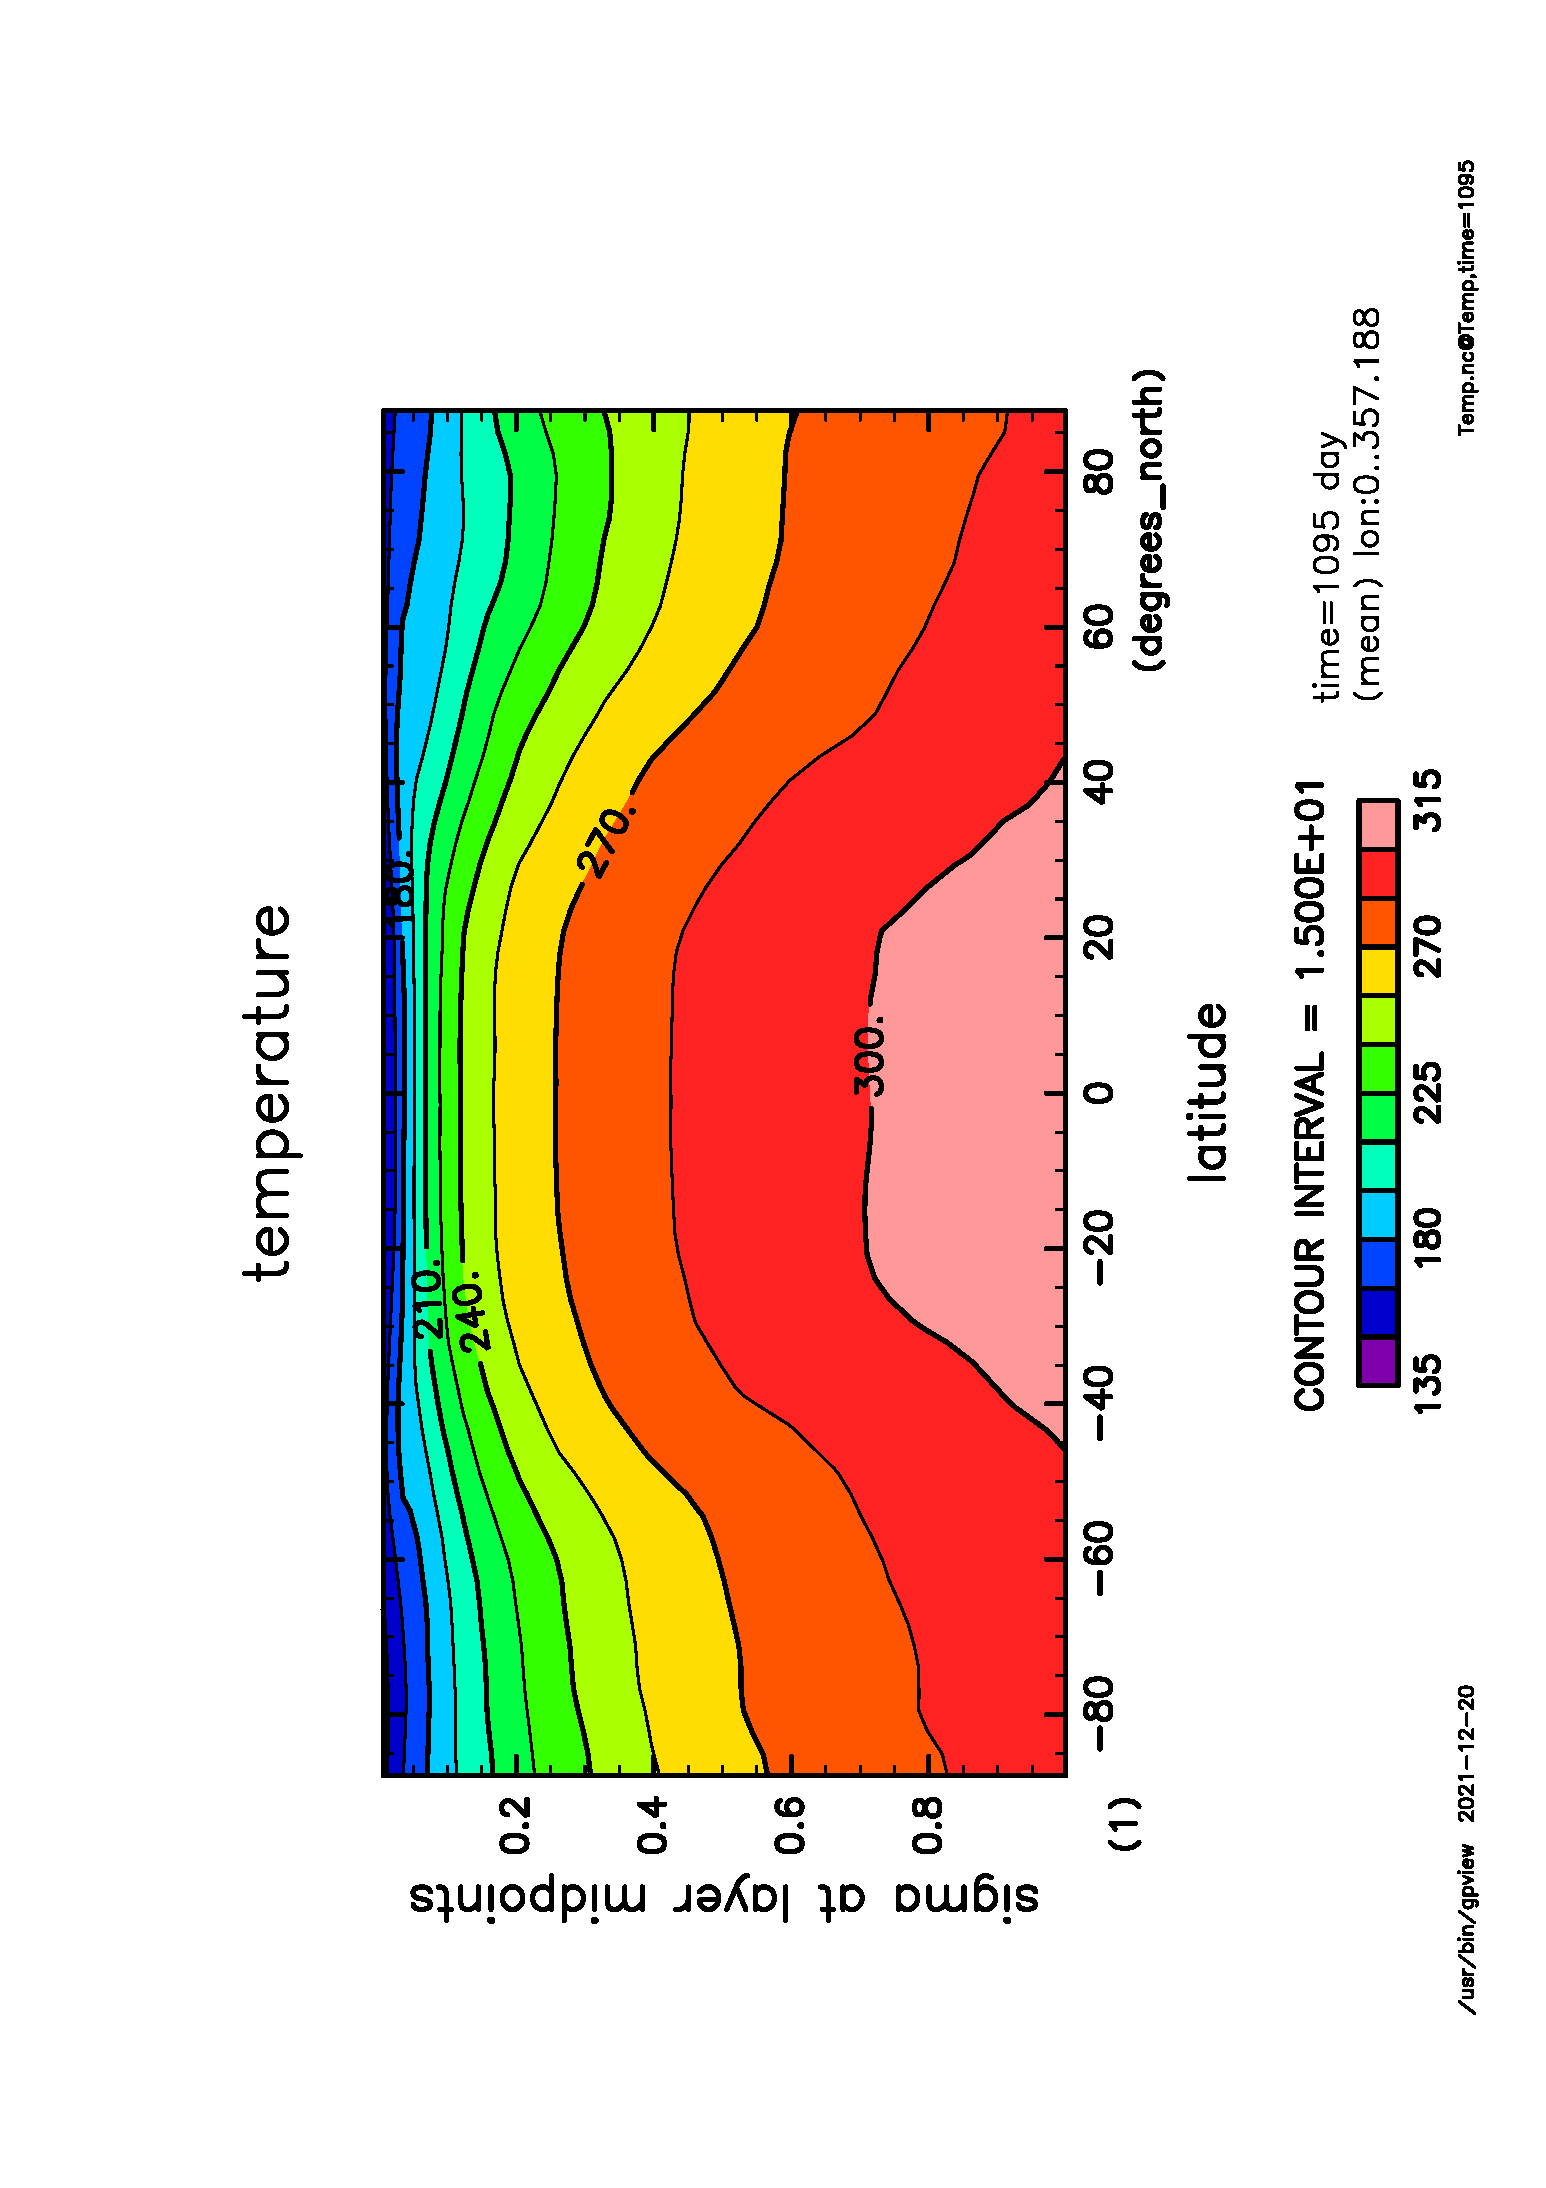
\includegraphics[height=\textwidth,angle=-90]{S2000Temp,time=1095.pdf}
	\caption{\(S=2000\hmu{W/m^2}\) 3 年目の子午面温度分布:w
	}
\end{figure}
\end{document}
